% !TeX root = ../main.tex
% Add the above to each chapter to make compiling the PDF easier in some editors.

\chapter{Related Works}\label{chapter:related_works}


\section{Fault feature extraction for DL-based Predictive Maintenance}

Nonstationary signal analysis is one of the main topics in the field of machinery fault diagnosis. Nonstationarity in this sense means that the signals change their statistical properties over time. Signals can consist of multiple frequencies and change their amplitude while traveling in time. Traditional signal analysis techniques make stationary assumptions. When applying those just statistical average in time or frequency can be extracted \cite{FENG2013}. The demand for analysis methods, which allows ascertain features of such nonstationary signal is increasing. These features help to collect machine health related information from the signals.

Traditionally, Fourier transforms are an important tool in signal analysis. The Fourier transform relates the one-dimensional time- and frequency domains as following:

\begin{equation}
    \begin{aligned}
        & time-domain (signal): \\
        & x(t) = \int_{f} X(f) e^{j 2 \pi t f} df \\
        & frequency-domain (spectrum): \\
        & X(f) = \int_{t} x(t) e^{- j 2 \pi f t} dt, \\
    \end{aligned}
\end{equation}

Since both domains are not combined but just related, the time specific information are lost in the frequency domain and the other way around. The relation between the time- and frequency domain created by the Fourier transformation is visualized in fig. \ref{fig:fourier} 
\begin{figure}[p]
  \centering
  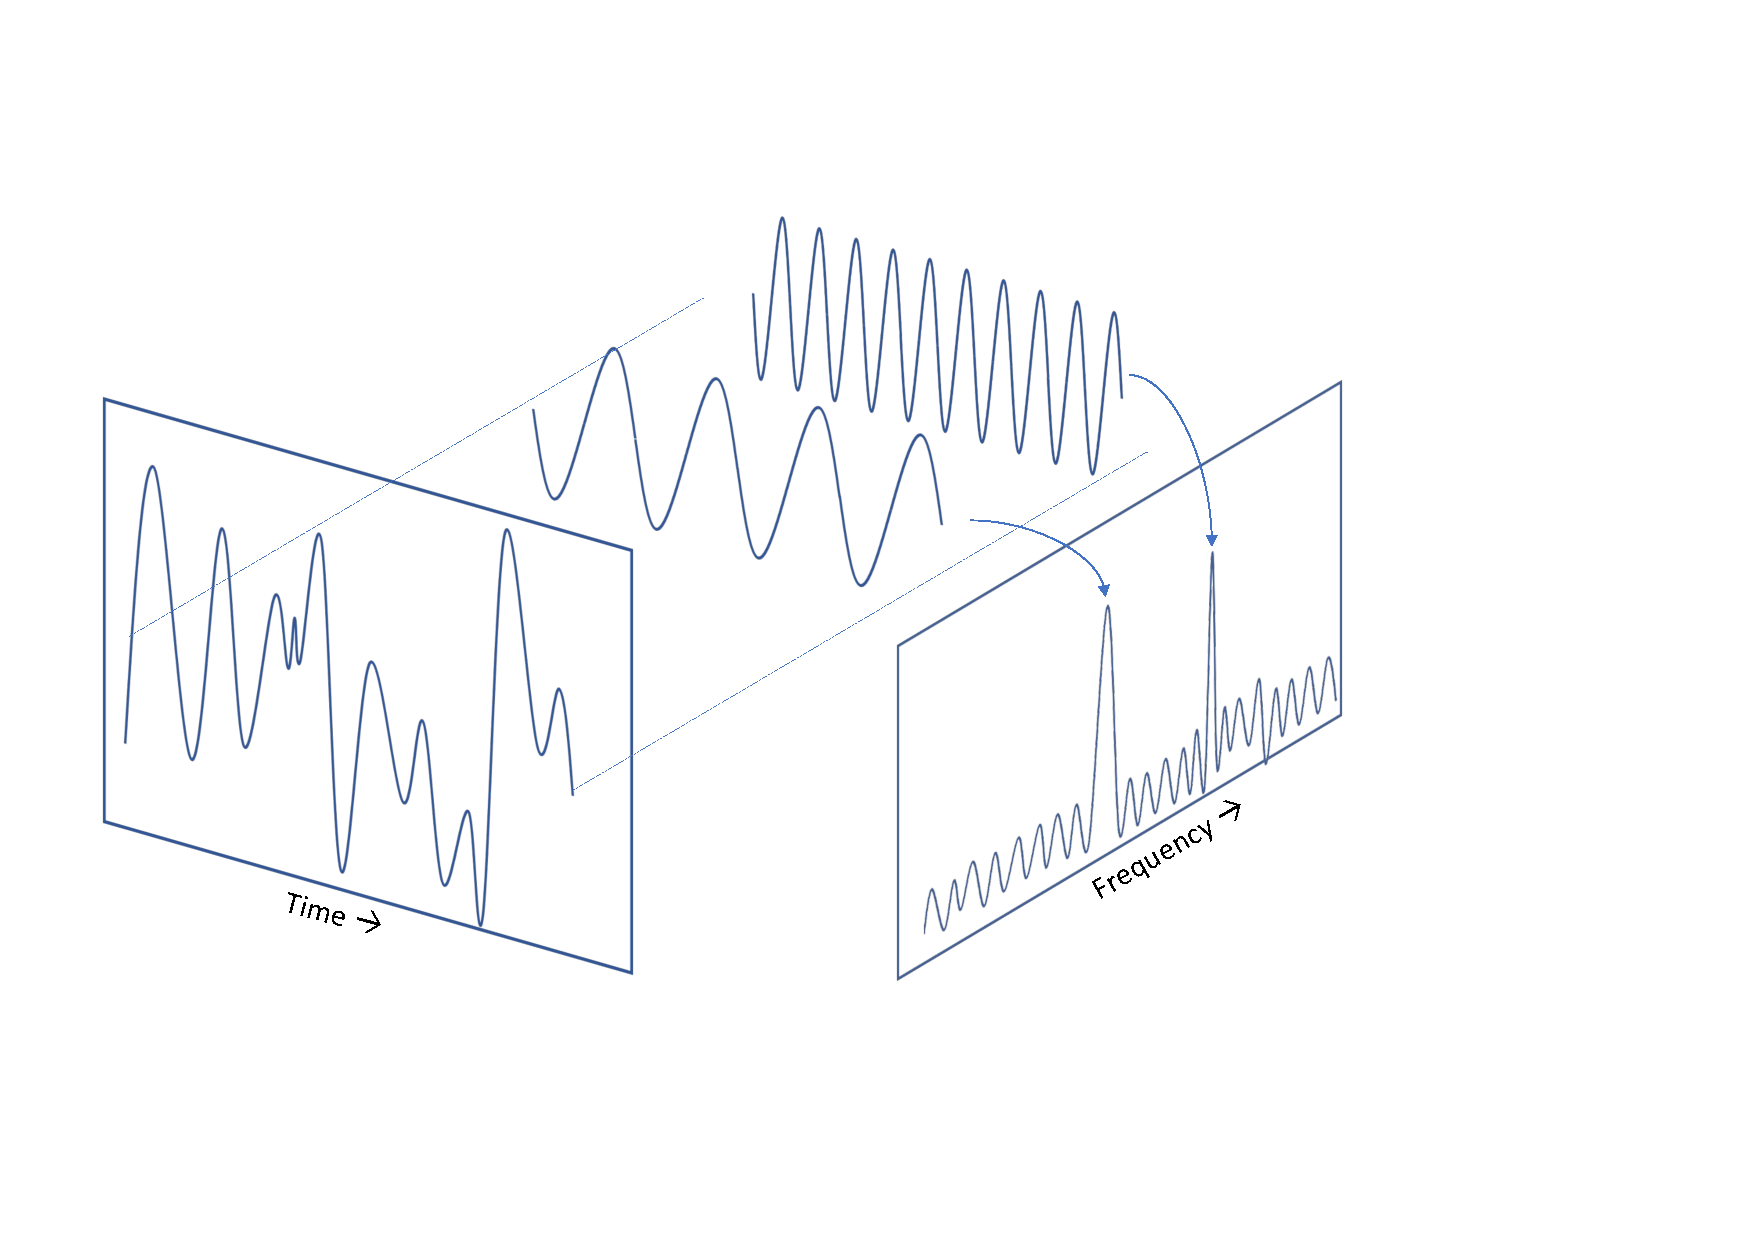
\includegraphics[width=.75\textwidth]{preprocessing_transform/fourier.pdf}
  \caption{Relation between time- and frequency domain through Fourier transformation}
  \label{fig:fourier}
\end{figure}

Time–frequency representations (TFR) solve this problem by transforming the one-dimensional signal in two-dimensional time-frequency plane, where each value corresponds to the dominance of a specific frequency at a certain point in time. Mathematically the two-dimensional data is represented by the joint function $T_{x}(f,t)$, where $x$ is the data of interest and the arguments of the function is the time  $t$ and frequency  $f$. One separates different methods of this type by the relation dependency of $T_{x}(f,t)$ on the input signal $x(t)$. There exit linear, quadratic or non-linear relationships.
The focus of this chapter is to describe linear and quadratic TFRs in more detail \cite{Hlawatsch1992}. 

\subsection{Linear time–frequency representations}
When the signal of interest can be decomposed in several linearly related components then the TFR of this signal can also be expressed as a linear combination of TFRs corresponding to each signal component:
\begin{equation}
    \begin{aligned}
        x(t) = c_{1} x_{1}(t) + c_{2} x_{2}(t) \rightarrow T_{x}(f,t) = c_{1} T_{x_{1}}(f,t) + c_{2} T_{x_{2}}(f,t)
    \end{aligned}
\end{equation}


All TFRs which fullfill this idea of linearity and superposition are called linear TFRs. The two most popular linear TFRs are the short-time Fourier and wavelet transform, which are presented in the following \cite{Hlawatsch1992}. 
\subsubsection{Short-time Fourier transform}

Short-time Fourier transform (STFT) is a method which adds a time variable to the traditional Fourier spectrum. This allows to investigate the variations in the signals spectrum over time. STFT assumes the signal's spectrum to be constant during a short time window. For each such window a Fourier spectrum is obtained and the time related changes are measured between such consecutive snapshots in the data. Window functions are defined which separate the signal. For each window a Fourier is applied. The process is mathematically expressed in the following:  
\begin{equation}
    STFT_{x}(t,f) = \int_{- \inf}^{+ \inf}x(\tau) w(\tau -t) exp(-j2\pi f \tau),
\end{equation}
where  $w(\tau -t)$ is the window function centered around t which is multiplied with the signal $x(t)$. Shifting the window over the signal and applying the Fourier transform $exp(-j2\pi f \tau)$ generates local spectra of the signal at for different points in time t \cite{FENG2013}. The time-frequency resolution is defined by the windowing function and the window length. STFT suffers from a trade-off between high resolution in time or in frequency but both at the same time is not possible. The optimum window length will depend on main interest behind the signal analysis. For accurate time domain information the window size needs to be reduced and for frequency domain information increased. STFT  decomposes the signal in existing sinusoidals and determines it's frequency and phase for a local part of the signal defined by the windowing function \cite{Hlawatsch1992}. 

\subsubsection{Wavelet transform}
The waveflet transform decomposes the signals in several wavelets which contain information about the health condition of the machine. A wavelet is a wave-like oscilation which is described by it's function, location and scale. The location defines where the wavelet overlaps with the signal and the scale defines how much squished (small scale) or streteched (big scale) the wavelet is. By changing the location of the wavelet it is shifted through the signal and overlaps with several different parts of the signal. While shifting the wavelet, it is multiplied with the signal  \cite{Shawhin2020}. The convolution of the wavelet and the signal is mathematically expressed in the following:
\begin{equation}
    WT_{x}(t,a) = \frac{1}{\sqrt{a}} \int_{- \inf}^{+ \inf} x(\tau) \psi(\frac{\tau -t}{a}) d \tau,
\end{equation}
 where $x(t)$ is the signal which is convolved with the wavelet $\psi(\frac{\tau -t}{a})$. In this case a is the scaling factor, t is the time shift and $frac{1}{\sqrt{a}}$ is a normalization factor to maintain the energy conservation \cite{FENG2013}. Different wavelet basis $\psi(t)$ can be convolved with the signal. This helps to analyze the signal for different pattern, which have similar properties as the wavelet \cite{Shawhin2020}. Possible wavelet basis could be the Gaussian, Morlet, Shannon, Meyer, Laplace, Hermit, or the Mexican Hat wavelets in both simple and complex functions \cite{Verstraete2017}. This allows a more extensive, flexible and detailed analysis. In fig. \ref{fig:ricker_wavelet} Ricker wavelets with different scales are visualized. Besides that wavelet transforms can extract local spectral and temporal information in parallel \cite{Shawhin2020}.


\begin{figure}[p]
  \centering
  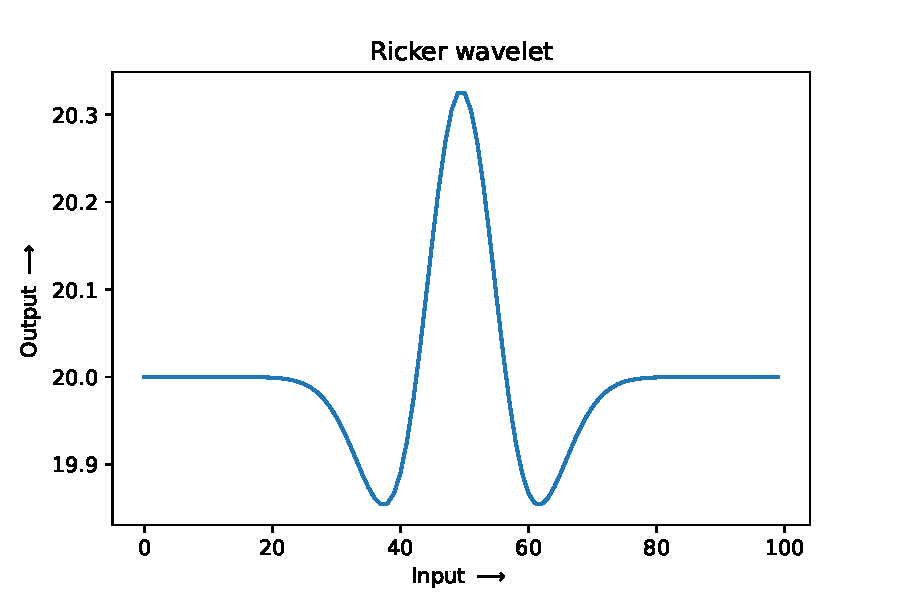
\includegraphics[width=.47\textwidth]{preprocessing_transform/wavelet_small_scale.pdf}
  \hspace{.1cm}
  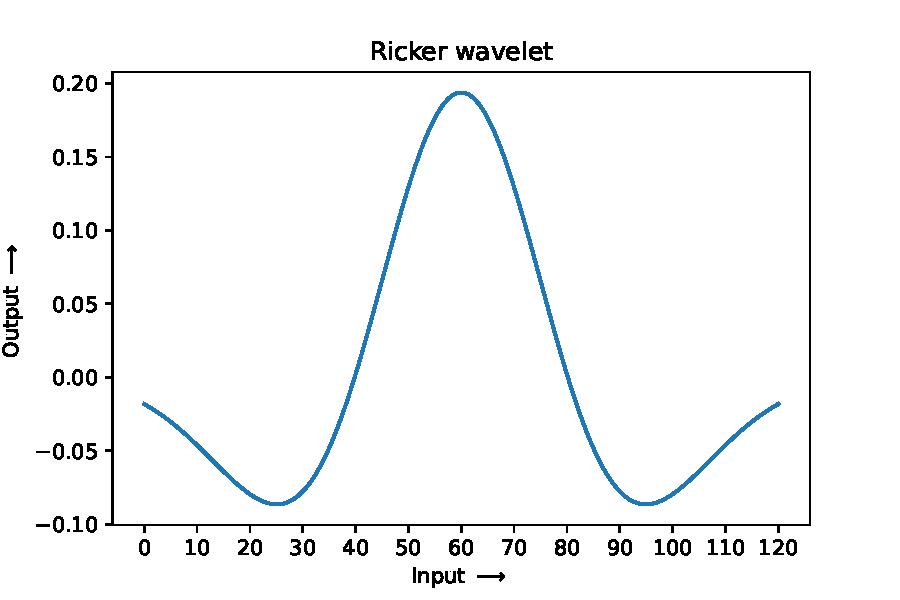
\includegraphics[width=.47\textwidth]{preprocessing_transform/wavelet_big_scale.pdf}
  
  \vspace{.1cm}
  
  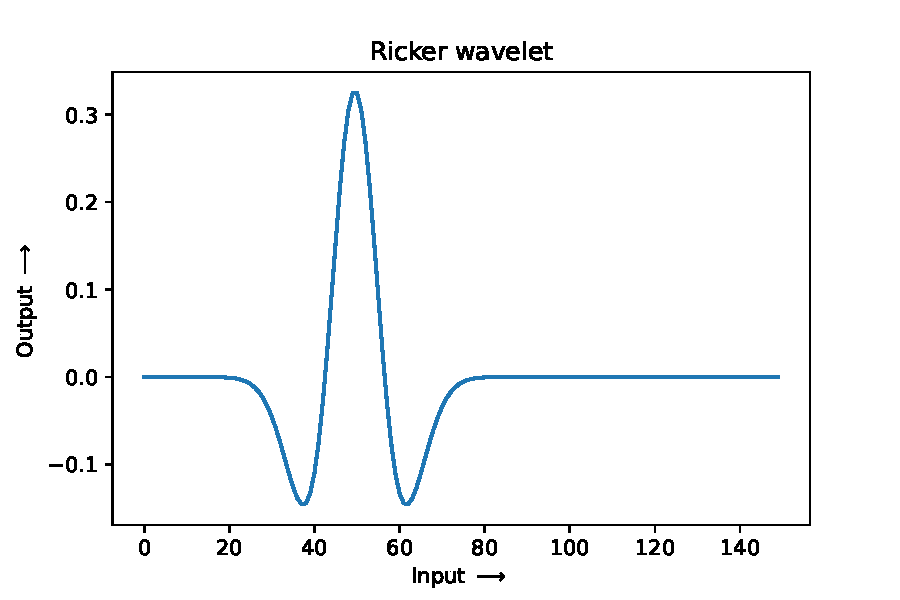
\includegraphics[width=.47\textwidth]{preprocessing_transform/wavelet_left_scale.pdf}
  \hspace{.1cm}
  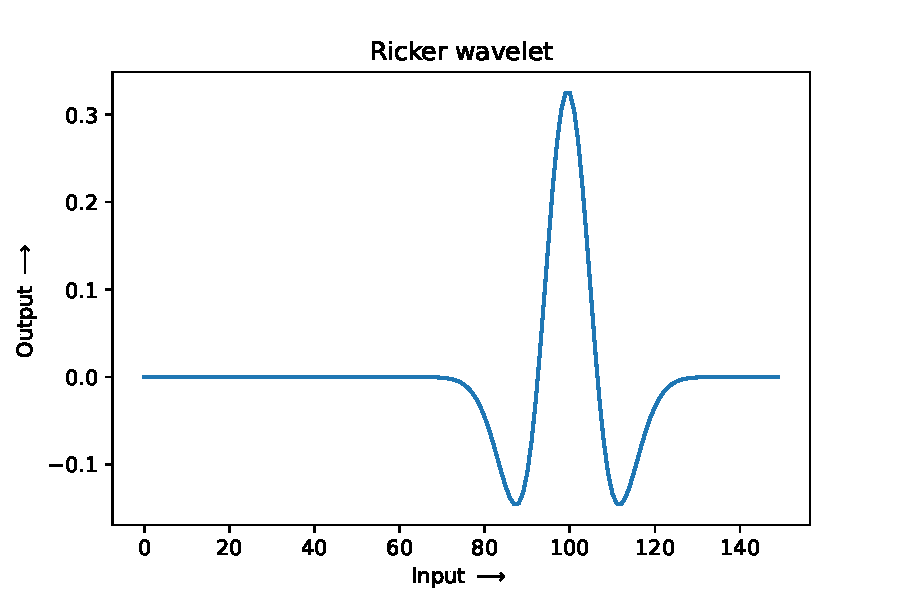
\includegraphics[width=.47\textwidth]{preprocessing_transform/wavelet_right_scale.pdf}

  \caption{Ricker wavelet with different scale (top) and shifting (bottom) factors}
  \label{fig:ricker_wavelet}
\end{figure}
\FloatBarrier 

\subsection{Spectrograms and Scalograms}

 Spectrograms are a graphic representation of the STFT and scalograms of the wavelet transform. Spectrograms and scalograms visualize the the squared magnitudes of the previously presented STFT and Wavelet transform. This squared magnitude are loosly interpreted as as signal energy \cite{Hlawatsch1992}. The mathematical expressions are presented in the following: 

\begin{equation}
    \begin{aligned}
        SPEC_{x}(t,f) = \abs{STFT_{x}(t,f)}^{2} \\
        SCAL_{x}(t,f) = \abs{WT{x}(t,f)}^{2}, 
    \end{aligned}
\end{equation}

where $STFT_{x}(t,f)$ is the Short-time Fourier transform, $WT_{x}(t,f)$ the wavelet transform, $SPEC_{x}(t,f)$ the spectrogram and $SCAL_{x}(t,f)$ the scalogram \cite{Hlawatsch1992}. This way of representing the system energy in the 2d time and frequency space may reveal useful information from the complex and high-dimensional data without the need for additional feature extraction. As described before spectrograms have a fixed frequency resolution that is defined by the windows size. Scalograms on the other hand have a frequency- dependent frequency resolution \cite{Verstraete2017}.

\subsection{Adaptive non-parametric time–frequency analysis}
Adaptive non-parametric approaches include empirical mode decomposition (EMD) \cite{FENG2013}. Unlike other multiresolution analysis (MRA) techniques such as wavelet analysis EMD recursively extracts Intrinsic Mode Functions (IMF) from a non-stationary time series. According to Faltermeier et al. \cite{Faltermeier2010} IMFs have the following properties: 

\begin{itemize}
    \item [1] An IMF has just one extremum between to zero crossings. Local minima and maxima do need to alternate such that the number of local minima and maxima does differ at most by one. 
    \item[2] An IMF need to have zero mean, but still the IMF can have changing frequencies and amplitude modulation. 
\end{itemize}

The EMD algorithm decomposes the signal as following:

\begin{equation}
    x(t) = \sum_{n} x_{n}(t) + r(t),
\end{equation}
where $x(t)$ is the signal, $x_{n}(t)$ the n-th IMF and $r(t)$ the residuum \cite{Faltermeier2010}. Faltermeier et al. \cite{Faltermeier2010} describte the recursive extraction of IMFs from the signal as following: 
\begin{itemize}
    \item [Step 0:] Initialize: $n := 1$, $r_{0}(t) = x(t)$
    \item [Step 1:] Extract the n-th IMF as follows:
    \begin{itemize}
         \item [a)] Set $h_{0}(t) := r_{n−1}(t)$ and $k := 1$
         \item [b)] Find all local maxima and minima of $h_{k−1}(t)$
         \item [c)] Construct envelopes for all the identified maxima $U_{k−1}(t)$and minima $L_{k−1}(t)$ for $h_{k−1}(t)$ using cubic interpolation
         \item [d)] Determine the mean $m_{k−1}(t) = 12 (U_{k−1}(t) - L_{k−1}(t))$ of both envelopes of $h_{k−1}(t)$.
         \item [c)] Form the k − th component $h_{k}(t) := h_{k−1}(t) - m_{k−1}(t)$
         \begin{itemize}
            \item [i)] if $h_{k}(t)$ is not in accord with all IMF criteria, increase $k \rightarrow k + 1$ and repeat starting at step b
            \item [ii)] if $h_{k}(t)$ satisfies the IMF criteria then set $x_{n}(t) := h_{k}(t)$ and $r_{n}(t) := r_{n-1}(t) − x_{n}(t)$
         \end{itemize}
    \end{itemize}
    \item [Step 2:] Check another IMF needs to be extracted
        \begin{itemize}
            \item [i)] if $r_{n}(t)$ is the residue, the original data is decomposed in the n IMFs  $x_{n}(t)$ and the residue $r_{n}(t)$
            \item [ii)] if $r_{n}(t)$ is not the residue, go to Step 1.
         \end{itemize}
\end{itemize}


The number of IMFs extracted roughly equls $log_{2}(N)$ where $N$ is the number of extrema in the signal. The EMD decomposes the non-stationary signal in its locally and non-overlapping component IMFs. This process does not need any predefined wave-forms like the wavelet transformations expects it. The selection of the IMFs is an automatic and adaptive time-variant filtering  \cite{Faltermeier2010}. Compared to the Fourier and Wavelet transform, the the decomposition of the signal in several IMFS does not divide the signal into fixed frequency components, which gives HHT a higher time-frequency resolution \cite{Verstraete2017}. The popular Hilbert-Huang Transform (HHT) combines the EMD with the Hilbert spectral analysis. For this each the Hilbert transform is applied to each of the detected IMFs. A corresponding analytical signal can be constructed. Also the Hilbert amplitude and energy spectrum can be derived. For more Hilbert-specific details Feng et al. \cite{FENG2013} can be studied.


\section{Domain adaptation approaches for Predictive Maintenance}

\subsection{Maximum Mean Discrepancy}
\subsection{Generative Adversarial Networks}

Since in this thesis Relu and Selu activation functions were mainly used in hidden and Softmax in final layer, those are described more in detail . The formula \ref{eq:relu} and \ref{eq:selu} show the definition of the Selu and Relu and \ref{eq:softmax} of the softmax activation functions: 

\begin{equation}
Selu(z) = \lambda
\left\{
\begin{matrix}
z \hspace{3.5em}, if \enspace z < 0\\
\alpha e^{z} - \alpha  \hspace{1em}, if \enspace z > 0.
\end{matrix}
\right.
\label{eq:selu}
\end{equation}

